% vi:ft=tex
\documentclass{standalone}

\usepackage{tikz}
\usepackage{verbatim}
\usepackage{mathtools}

\usetikzlibrary{arrows}
\usetikzlibrary{calc}

\begin{document}

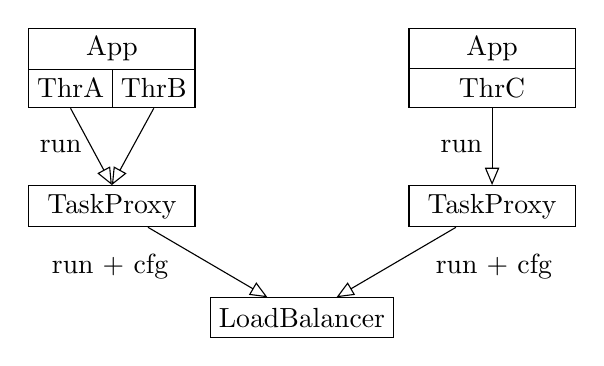
\begin{tikzpicture}[node distance=2.0cm]

  % Colors
  % Styles
  \tikzstyle{defaultRec} = [text centered, inner sep = 3pt,
    draw=none, shape=rectangle, fill=white, minimum height = .5cm, minimum
  width = 1.4cm];
  \tikzstyle{tpRec} = [defaultRec, draw=black,text width=1.9cm];
  \tikzstyle{threadRec} = [defaultRec, draw=black, node distance=0mm,
  minimum width=1cm]
  \tikzstyle{arrow} = [-open triangle 45, black];

  % Variables

  % Drawing

  \node(tm) [defaultRec, draw] at (0, 3) {LoadBalancer};

  \node(tp1) [tpRec, above left of=tm,xshift=-1cm] {TaskProxy};
  \draw[transparent] (tp1.west) -- +(0,15mm) coordinate(helpWest);
  \node(t1-1) [threadRec, right of=helpWest,anchor=west,] {ThrA};

  \draw[transparent] (tp1.east) -- +(0,15mm) coordinate(helpEast);
  \node(t1-2) [threadRec, right of=helpEast,anchor=east,] {ThrB};

  \node(a1)	[tpRec, above of=tp1, node distance=2cm] {App};
  \draw [arrow] (t1-1.south) -- node[midway,anchor=east]{run} (tp1.north);
  \draw [arrow] (t1-2.south) -- (tp1.north);

  \node(tp2) [tpRec, above right of=tm,xshift=1cm] {TaskProxy};
  \node(a2)	[tpRec, above of=tp2, node distance=2cm] {App};
  \node(t2) [threadRec, below of=a2,node distance=5mm, text width=1.9cm] {ThrC};
  \draw [arrow] (t2.south) -- node[midway, anchor=east] {run} (tp2.north);

  \draw [arrow] (tp1) -- node[near start,below, anchor=north east]{run + cfg} (tm);
  \draw [arrow] (tp2) -- node[near start,below, anchor=north west]{run + cfg} (tm);

\end{tikzpicture}

\end{document}
